\documentclass[a4paper,10pt]{article}

\usepackage[utf8]{inputenc}
\usepackage[T1]{fontenc}
\usepackage[french]{babel}
\usepackage{geometry}
\usepackage{a4wide}
\usepackage{fullpage}
\usepackage{enumerate}
\usepackage{amsmath, amsfonts, amstext, amssymb}
\usepackage{tikz}
\usetikzlibrary{decorations,decorations.pathmorphing,decorations.pathreplacing}

\usetikzlibrary{shapes.misc}
\newcommand*\quartgauche{{\tikz{\draw[->] (0,0) arc (0:90:.2);}}}
\newcommand*\quartdroit{{\tikz{\draw[->] (0,0) arc (180:90:.2);}}}
\usepackage{tikzsymbols}

\usepackage{xspace}% espace intelligent pour les macros
\newcounter{ctr_exercices}
\newcommand{\doublerulefill}{
\rule{\textwidth}{3pt}
\rule[3mm]{\textwidth}{0.5pt}
}\newcommand{\exercice}[1]{
\refstepcounter{ctr_exercices} % "ref"stepcounter pour pouvoir faire
                               % des \ref sur le numero d'exercice
\section*{\'Etape \arabic{ctr_exercices}~\hrulefill~{#1}}}
\renewcommand{\fup}{$\uparrow$\xspace}
\newcommand{\fdo}{$\downarrow$\xspace}
\newcommand{\fle}{$\leftarrow$\xspace}
\newcommand{\fri}{$\rightarrow$\xspace}
\newcommand{\tri}{\quartdroit\xspace}
\newcommand{\tle}{\quartgauche\xspace}


\begin{document}
\pagestyle{empty}

\begin{center}
{\large \bf Les marmottes au sommeil léger}
\smallskip
{... une idée farfelue de Marie Duflot-Kremer}
\end{center}
\doublerulefill


Le document que vous êtes en train de consulter n'est pas une
référence très finalisée, ni un guide strict à suivre. Il regroupe des
infos que vous pourriez trouver utiles si vous envisagez d'animer
cette activité. Il contient l'histoire des marmottes, le déroulé de
l'activité, l'explication côté informatique ainsi qu'un patron à
imprimer pour réaliser l'activité. La diffusion de
ce document est libre, vous pouvez suggérer des
améliorations/enrichissements à
\verb=marie.duflot-kremer@loria.fr=. Si ce document vous a été utile,
vous pouvez également me le signaler car
j'envisage de mentionner sur ma page médiation les
écoles/associations/etc. qui ont testé et approuvé l'activité. La page
\verb=https://members.loria.fr/MDuflot/= permet de trouver (section
médiation/activités) une liste d'autres activités pour faire découvrir
différents aspects de l'informatique, réalisables en grande majorité
sans ordinateur.

\exercice{Le contexte}

Un groupe de marmottes, moyennement satisfaites de leur terrier
actuel, décide de concevoir un nouveau terrier et de le
creuser avant l'hiver. Pour ce faire les marmottes doivent respecter
trois règles.
\begin{enumerate}
\item A partir de l'entrée on peut construire deux couloirs,
et au bout de chaque couloir on peut faire un embranchement vers deux
autres, mais pas plus (au risque de faire s'écrouler l'édifice).
\item Les marmottes vont chacune occuper une salle différente (pour ne
  pas se réveiller les unes les autres) et forcément une salle qui est
  tout au bout d'un couloir. Pour des marmottes au sommeil léger il
  est inenvisageable de dormir dans une salle à un embranchement, car
  les marmottes qui seraient au-delà de cet embranchement leur
  marcheraient dessus en entrant/sortant, et cela ruinerait leur
  hibernation
\item Chaque marmotte se réveille un nombre précis de fois dans
  l'hiver, et s'il n'est pas grave de mettre assez loin de l'entrée une marmotte qui ne se
  réveille (et donc ne sort du terrier) qu'une fois dans l'hiver,
  c'est bien plus embêtant de mettre loin une marmotte qui va se
  réveiller 10 fois par exemple. Comme les pas de marmottes émettent
  de légères vibrations et que nos marmottes ont vraiment le sommeil
  léger, on va vouloir minimiser les déplacement de l'ensemble du
  groupe. Pour cela on va compter les déplacements de la façon
  suivante. Une marmotte dormant à 4 couloirs de l'entrée se réveillant 5 fois
  dans l'hiver va parcourir 4 x 5 = 20 couloirs aller et retour (pour
  simplifier on ne va compter que les allers). On va faire la somme
  des déplacements de toutes les marmottes et essayer de rendre cette
  somme la plus petite possible.
\end{enumerate}

\exercice{Préparer le matériel}

Avec le modèle de couloirs et de marmottes donné, on peut préparer un
kit. Pour cela il vous faut une imprimante, un stylo, des ciseaux, une plastifieuse
et des feuilles plastiques qui vont avec, et un peu de scratch adhésif
(se trouve en mercerie). Ensuite il vous suffit de : 
\begin{itemize}
\item tout imprimer,
\item découper couloirs et marmottes (pour les marmottes laisser un
  peu de place autour, qui représente la salle dans laquelle elle dort),
\item ecrire des 0 (branche de gauche) et des 1 (branche de droite) 
  \underline{au dos} des couloirs,
\item choisir une phrase à compresser ne contenant pas plus de 8
  caractères différents (sinon il nous faut plusieurs planches pour un
  kit) et compter la fréquence d'apparition des caractères (espace
  compris),
\item noter au dos de chaque marmotte un des caractères et sa fréquence
  (par exemple A 6) et recopier la fréquence côté marmotte (c'est le
  nombre de fois où elle se réveille pendant l'hiver)
\item plastifier le tout (marmottes + couloirs) et redécouper en
  laissant un peu de marge pour que cela tienne bien,
\item placer de petits morceaux de scratch adhésif de la façon
  suivante :
  \begin{itemize}
  \item des morceaux tout doux au dos du coude des couloirs et au dos
    des marmottes (sans cacher la lettre qui y est écrite !)
  \item des morceaux grattants côté recto aux extrémités des couloirs
  \end{itemize}
\end{itemize}

Pour un (des ?) exemple de phrase et de de nombres à écrire aller voir la section sur l'explication
informatique.

La plastification se fait ici une fois les éléments découpés pour que
le plastique soit bien scellé sur les bords de chaque objet.

\exercice{Et maintenant, creusez}

Pour commencer on va distribuer des kits et expliquer les règles
ci-dessus. Les participants peuvent donc expérimenter et créer
eux-mêmes leurs terriers, en essayant d'avoir le meilleur
possible. L'animateur doit donc avoir résolu le problème avant et
savoir dire au vu d'un terrier s'il est optimal ou non (la bonne
nouvelle c'est qu'on peut lire d'abord la suite et avoir l'algo qui
donne le nombre de déplacements minimal).

Pour compter le nombre de déplacements au total, on a deux solutions :
\begin{itemize}
\item pour chaque marmotte, calculer sa distance jusqu'à l'entrée,
  faire la multiplication avec le nombre de fois qu'elle se réveille
  dans l'hiver, puis faire la somme de tous ces résultats
\item ... ou bien, on peut calculer pour chaque pièce de couloir
  combien de fois elle est traversée. Par exemple, un couloir qui
  relie deux marmottes se réveillant respectivement 5 et 2 fois, on
  note dans le coude du couloir la valeur 5 + 2 = 7. Si un couloir
  relie maintenant une marmotte se réveillant 4 fois et le couloir
  précédent (qui porte donc la valeur 7), on note sur son coude la
  valeur 7 + 4 = 11. On continue jusqu'à l'entrée du terrier, puis il
  reste juste à faire la somme de tous les chiffres écrits dans les couloirs.
\end{itemize}

Le point positif est qu'on ne peut pas vraiment se "tromper" en faisant cette
étape, on finit par avoir un terrier, et puis on essaie de le
transformer pour l'améliorer. 

\exercice{Comment trouver le meilleur terrier ?}

Pour trouver le meilleur terrier, il y a une méthode infaillible, qui
ne demande pas trop de calculs : 
\begin{itemize}
\item on choisit les deux (ou deux parmi les) marmottes qui se lèvent
  le moins souvent, et on les relie par un morceau de terrier. Sur le
  coude on note le nombre de fois que ce morceau est emprunté (donc la
  somme des valeurs des deux marmottes, par exemple 2 + 3 = 5)
\item on recommence exactement la même chose, mais les deux marmottes
  reliées à l'étape précédente comptent maintenant pour une seule marmotte qui se
  réveillerait 5 fois 
\item on continue, jusqu'à ce que toutes les marmottes soient reliées
  en un seul terrier.
\item et comme on a noté des chiffres sur les coudes de terriers au fur
  et à mesure on a juste à faire la somme de ces chiffres pour compter
  le nombre de déplacements 
\end{itemize}


\exercice{Et hop, c'est de l'informatique}

Oui bon c'est bien sympa tout ça mais quel est le rapport avec
l'informatique ? C'est juste qu'on a suivi un algorithme pour faire le
meilleur terrier ? Eh non, parce que cet algorithme n'aide pas que les
marmottes (en fait il n'est même pas prouvé qu'il les aide) mais est
utilisé dans le domaine de la compression de texte.

C'est là qu'on retourne les terriers (qui tiennent si on a bien mis
les scratchs) et qu'on découvre la version informatique du
problème. La structure que l'on obtient est celle d'un arbre, avec
(oui les informaticiens sont des blagueurs) la racine en haut, les
couloirs qui se nomment des branches, et les extrémités des branches
appelées feuilles. Et dans cet arbre une marmotte correspond à une lettre, et son nombre de
réveils au nombre de fois que la lettre apparaît dans un texte. 

Par exemple dans la phrase BARBARA RASE BASILE LE BARBIER, il y a 6 A,
5 B, 4 espace etc. qui seraient au dos de marmottes se réveillant, 6,
5 et 4 fois. 

Le but de la compression est de trouver un codage du texte, en binaire parce
que dans un ordinateur tout est stocké en binaire, qui soit le plus
court possible, et qui soit facile à coder et décoder. En général pour
représenter un texte non compressé, on utilise le code ASCII ou l'une
de ses extensions. Mais même rien qu'en ASCII on a 8 chiffres binaires
(8 bits) pour stocker un caractère. Si ce n'est pas grave que le code
du "w" ou du "k" soient longs en français, par contre le "e" qui
apparaît plus souvent on aimerait bien que son code soit plus court,
et c'est précisément ce que fait le codage de Huffman : donner à
chaque lettre un code binaire tel que si on met bout à bout le code de
toutes les lettre du texte, on a une version codée la plus courte possible.

Sur notre structure de terrier on peut facilement lire le code de
chaque lettre : on part de la racine du terrier et on lit le bit écrit
sur chaque couloir que l'on emprunte (cf section matériel). Par
exemple si pour aller de l'entrée à la lettre A on prend à gauche
puis à droite puis à droite, le code de A est 011.

Les trois contraintes que l'on a imposées sur les terriers se justifient quand on veut
faire de la compression de texte. La preuve ci-dessous : 

\begin{itemize}
\item tout d'abord minimiser le nombre de déplacements dans le terrier
  correspond exactement à minimiser la taille du texte en binaire. On
  aura autant de chiffres binaires pour coder tout le texte qu'on
  avait de déplacement de marmottes dans les couloirs (si on a compté
  les allers et pas les retours),
\item ensuite on n'autorisait pas plus de deux nouveaux couloirs partant de
  l'entrée ou du bout d'un couloir. Cela correspond au binaire. Comme
  on a deux valeurs à mettre sur les couloirs à chaque étape (0 et 1),
  on ne peut avoir que deux couloirs qui partent,
\item enfin il était interdit de mettre une marmotte dans une salle
  d'où partent de nouveaux couloirs, car ce la la réveillerait. Côté
  informatique cette propriété que l'on impose (les marmottes en bout
  de couloirs) correspond à un codage préfixe (voir ci-dessous).
\end{itemize}

Imaginez que je donne le code 0 à la lettre E, 01 à la lettre S  et 10
à la lettre T. Pour coder ce n'est pas difficile : ETES donne 0 puis
10 puis 0 puis 01 soit 010001. Par contre pour décoder c'est
franchement plus difficile. Si je lis 10010001 je sais que ça commence
par un T, et puis il me reste 010001 que je peux décoder en ETES ou
SEES. Sur cet exemple je sais que TETES est un mot et TSEES pas, mais
sur un long texte je vais au mieux perdre \underline{énormément} de
temps, au pire avoir plusieurs possibilités et ne pas savoir comment
décoder. 

Le problème est que 0 est à la fois le code de E et le début du code
de S, donc si je vois un 0 je ne sais pas si je peux décoder E tout de
suite ou prendre le prochain bit et les décoder ensemble. Si au
contraire on impose un codage préfixe, on va commencer à la racine,
suivre les branches en fonction des 0 et 1 dans le texte compressé, et
dès qu'on arrive sur une lettre on la note (comme on ne peut pas
continuer plus loin car la branche s'arrête là, on est sûr d'avoir lu le
code de cette lettre) et on repart de la racine en continuant à lire
les chiffres binaires. Le décodage/décompression se fait donc très
rapidement et sans hésitation.
 
Pour donner un exemple d'efficacité, sur le texte intégral de Cyrano
de Bergerac, le gain obtenu en passant du texte (codé en UTF-8) non
compressé à la version compressée avec la méthode ci-dessus est de
40\%. On a donc diminué quasiment de moitié la taille du texte, rien
qu'avec un algorithme explicable à des enfants. 

Et les codes qui ne sont pas préfixes, on peut les jeter ? Non, pas
tous. Si on regarde le code Morse par exemple, on a le E (un point)
qui est préfixe du I (deux points). La différence c'est qu'en Morse on
fait une légère pause entre deux lettres qui permet de savoir quand
une lettre s'arrête et ainsi différencier un double e d'un i. En
informatique tous les à et les 1 sont rangés les uns à la suite des
autres, sans pause, et c'est pour cela qu'on a besoin d'un codage préfixe.

\exercice{Et en vrai, comment ça se passe ?}

Cette activité a pour moi plusieurs avantages. Le côté ludique des
marmottes aide à se projeter et entrer dans l'activité, mais ce n'est
pas tout. 
\begin{itemize}
\item tout d'abord l'algorithme de compression présenté n'est pas un
  algorithme jouet conçu exprès pour ça mais un véritable algorithme
  de compression, inventé par David Albert Huffman en 1952, alors
  doctorant au MIT,
\item et cet algorithme a la particularité d'être optimal, c'est à
  dire que si on donne un code binaire à chaque lettre on ne peut pas
  faire mieux que le taux de compression obtenu avec l'algorithme de
  Huffman,
\item et enfin, et cela ne gâche rien, l'algorithme de Huffman est
  toujours utilisé, plus de 60 ans plus tard. On ne l'utilise pas
  seul, mais les formats compressés que l'on connaît : zip pour
  notamment les fichiers texte, mp3 pour le son, mp4 pour la vidéo
  etc, utilisent l'algorithme de Huffman. Il se composent en
  général d'une première étape, plus complexe et dépendante du type
  d'information à compresser (image, son, texte), suivie par une
  application du codage de Huffman.
\end{itemize}

Un dernier point. Si l'algorithme de Huffman est optimal, pourquoi
fait-on une autre étape de compression aux fichiers texte ? En fait le
codage de Huffman est le meilleur quand on impose d'associer un code à
chaque lettre. Si on veut faire mieux, l'idée est, avant d'appliquer
Huffman, de décider à quels blocs du texte on va associer des
codes. En français par exemble, les digrammes (blocs de 2 lettres)
"es", "en" ou "le" sont les plus fréquents. Il est donc plus efficace
de choisir un code pour "es" plutôt que de le coder avec le code de "e"
plus celui de "s". Et c'est en codant plusieurs lettres d'un coup que
l'on peut aller plus loin que l'algorithme de Huffman dans la
compression de textes.
\newpage
\thispagestyle{empty}
\hspace*{-1.5cm}\begin{tikzpicture}
  \node[] (marmottes) at (9,13) {\hspace*{-1.5cm}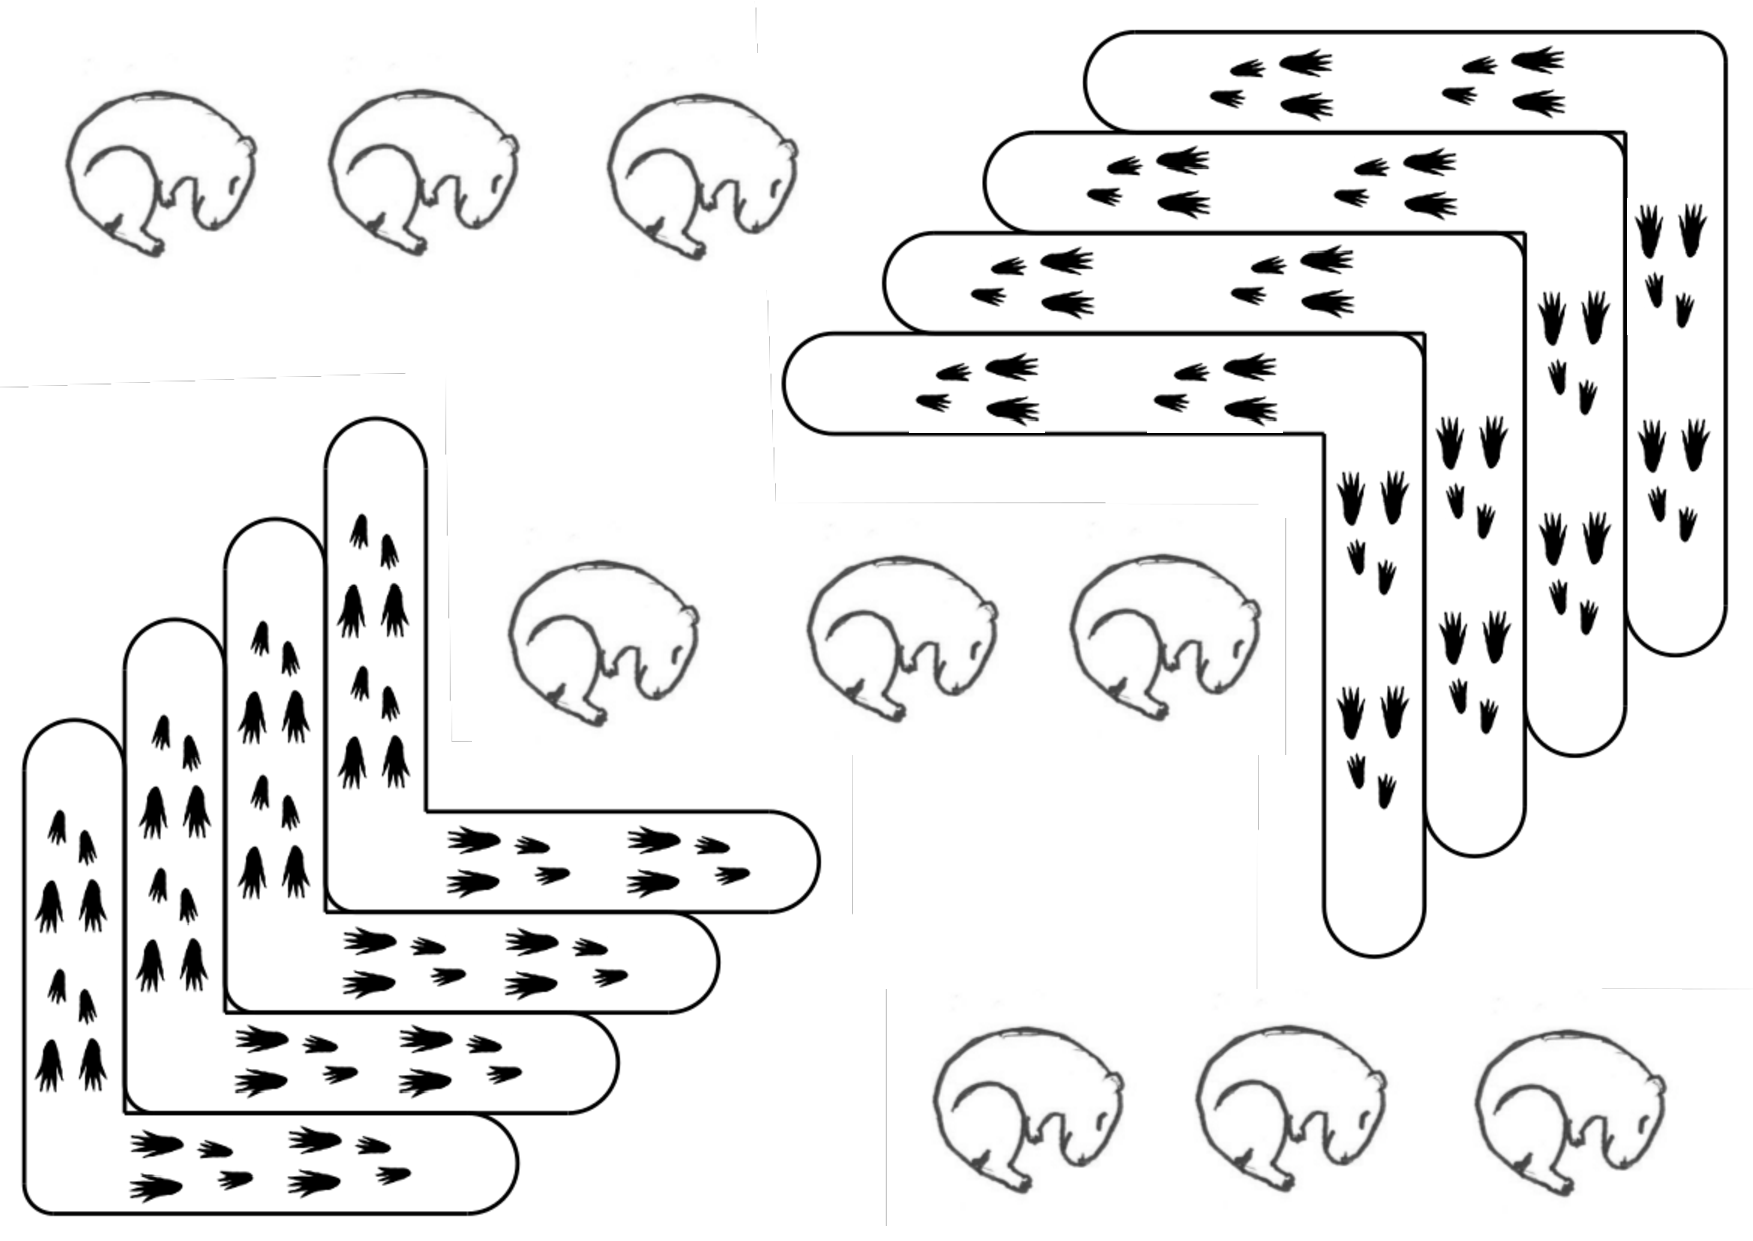
\includegraphics[angle=90,width=180mm]{complet.pdf}};
  \node[rotate=90] (info) at (-0.7,13) {plus informations (en français) sur {\tt https://members.loria.fr/MDuflot/} rubrique Médiation/Activités};
\end{tikzpicture}
\end{document}
